\documentclass[10pt,twocolumn]{article}

\usepackage[utf8]{inputenc}
\usepackage[margin=0.75in]{geometry}
\usepackage{amsmath,amssymb,amsfonts}
\usepackage{graphicx}
\usepackage{booktabs}
\usepackage{cite}
\usepackage{url}
\usepackage{microtype}
\usepackage{hyperref}

\hypersetup{
    colorlinks=true,
    linkcolor=blue,
    citecolor=blue,
    urlcolor=blue
}

\title{Auditable Failure Memory for ROS 2 Navigation:\\An Exploratory Comparison with Spatial Caching}

% Venue-Neutral Author and Grant Placeholders
% Authors: Replace placeholders with institutional names and grant identifiers upon venue selection
\author{
    Author One\thanks{Department of Robotics, University Placeholder. Correspondence to: \texttt{author.one@example.edu}}
    \and
    Author Two\thanks{Department of Computer Science, Institute Placeholder.}
    \and
    Author Three\thanks{Autonomous Systems Laboratory, University Placeholder.}
}
\date{}

\begin{document}

\maketitle

\begin{abstract}
In multi-phase indoor robot navigation, reactive navigation systems lacking cross-phase memory repeatedly re-enter occluded dead-end corridors across sequential tasks when initial line-of-sight is obstructed. We present \textbf{FailMem}, an event-driven failure memory architecture for ROS~2 Nav2 that binds navigation aborts to immutable observation bundles---combining raw LiDAR scans, coordinate transforms, and local costmap regions of interest---and provides perception-driven dynamic invalidation when clearance is verified by sensors. Within an asymmetric dual-path environment in Gazebo~11 simulations with a TurtleBot3 robot, we evaluate FailMem across 30 Gazebo simulation runs ($n=3$ per condition under sequential fixed seeds) against reactive retry ($R$), persistent suppression ($M1$), and spatial observation caching ($O$) baselines, alongside an exploratory 4-run feasibility trial on action-conditioned navigation ($H_1$). Memory retention and invalidation are evaluated across sequential phases within a single continuous runner execution session. The evaluation demonstrates that cross-phase memory successfully prevents redundant dead-end exploration in obstructed settings, and dynamic invalidation unsuppresses the shorter route upon blockage removal (reducing travel distance by $\approx 11.0\%$ relative to permanent suppression, though total episode duration showed no observed improvement). Under static 2D geometry, FailMem and spatial caching chose identical topological routes with under $1\%$ difference in distance and duration, showing no additional routing benefit of FailMem over spatial caching in the evaluated layout and run sample. Furthermore, candidate action configurations in $H_1$ did not establish the expected executability divergence (Nav2 returned success in 4/4 runs, with strict physical arrival verified in 3/4 runs; the candidate scenario did not establish the expected executability divergence).
\end{abstract}

\section{Introduction}
Autonomous mobile robots operating in structured indoor facilities---such as warehouses, hospitals, and office corridors---frequently encounter unmapped or transient physical blockages (such as parked delivery carts or closed safety doors) along nominal routes. Standard navigation systems, including the ROS 2 Navigation Stack (Nav2) \cite{macenski2020marathon2, macenski2022ros2}, utilize layered 2D costmaps \cite{lu2014layered} and local recovery behaviors (e.g., in-place rotations, backup maneuvers, costmap clearing). In standard Nav2 configurations, navigation actions are dispatched independently, and recovery routines operate within the lifetime of an individual goal execution \cite{macenski2020marathon2}. Consequently, when goals are dispatched sequentially from a distant decision junction without cross-goal memory, a purely reactive agent re-enters known dead ends until on-board sensors re-acquire line-of-sight to the blockage.

To mitigate unguided re-exploration, two primary approaches exist:
\begin{enumerate}
    \item \textbf{Spatial Costmap Caching ($O$)}: Maintaining geometric occupancy in persistent global grids (e.g., Costmap2D \cite{lu2014layered}, OctoMap \cite{hornung2013octomap}, Voxblox \cite{oleynikova2017voxblox}) as sensory observations accumulate.
    \item \textbf{Episodic Failure Memory ($F$)}: Recording explicit execution aborts, error causes, or symbolic constraints to suppress infeasible route options in high-level dispatching.
\end{enumerate}

While embodied AI frameworks explore language-based reflection (e.g., Reflexion \cite{shinn2023reflexion}, REFLECT \cite{liu2023reflect}), they are designed for high-level semantic task planning and verbal reflection. In mobile robot navigation, where spatial occupancy is continuously tracked in metric grids, integrating discrete execution failures with sensor-verified invalidation requires explicit coordination with perception. This raises an empirical question: \emph{Under what conditions does an autonomous mobile robot genuinely require explicit episodic failure memory over standard spatial costmap caching?}

In this work, we present \textbf{FailMem}, an event-driven failure memory architecture for ROS 2 Nav2, and conduct an exploratory empirical study to delineate its operational boundaries. Specifically, we provide:
\begin{enumerate}
    \item \textbf{Perception-Grounded Event Memory and Dynamic Invalidation Implementation}: A ROS 2 Nav2 architecture that binds execution aborts to immutable observation bundles (raw LiDAR scans, TF transforms, costmap ROIs) and executes sensor-verified dynamic invalidation upon clearing.
    \item \textbf{Auditable Exploratory Navigation Comparison}: A reproducible 30-run benchmark ($n=3$ per condition under sequential fixed seeds) in Gazebo 11 simulation runs comparing FailMem ($F$) against reactive ($R$), spatial caching ($O$), and persistent suppression ($M1$) baselines across clean (D0), blocked (D1), and restored (D2) scenarios.
    \item \textbf{Boundary Findings on Failure Memory vs. Spatial Caching}: An empirical finding that within the evaluated static 2D hallway layout, specific implementation, and run sample ($n=3$), FailMem yields no observed routing benefit over spatial caching ($O$), selecting identical topological routes ($<1\%$ difference in distance and duration); alongside empirical stopping criteria from an exploratory 4-run feasibility trial where action-conditioned navigation ($H_1$) did not establish executability divergence (Nav2 returned success in 4/4 runs, with strict physical arrival verified in 3/4 runs, without establishing the expected executability divergence).
\end{enumerate}


\section{Related Work \& Mechanism Taxonomy}
\subsection{Spatial Occupancy Mapping \& Distance Fields}
Layered 2D costmaps \cite{lu2014layered, macenski2020marathon2} maintain geometric obstacles by ray-casting sensor ranges into grid cells and propagating configuration-space inflation. 3D volumetric frameworks, such as OctoMap \cite{hornung2013octomap}, employ hierarchical octrees with discrete probabilistic voxel occupancy updates. Distance-field frameworks such as Voxblox \cite{oleynikova2017voxblox} incrementally construct continuous Euclidean Signed Distance Fields (ESDF) for smooth trajectory optimization. These mapping representations are fundamentally designed to track geometric occupancy and distance fields from sensor rays. Because their core primitive is geometric spatial state rather than execution history, they do not inherently index episodic navigation action aborts or high-level failure metadata.

\subsection{Execution Monitoring \& Plan Diagnosis}
Deliberative robotics frameworks \cite{fikes1971strips, simmons1998xavier, ingrand2017deliberation} formalize plan execution monitoring and diagnostic repair. Modern navigation stacks, including Nav2 \cite{macenski2020marathon2}, execute local recovery behaviors (such as in-place rotations, costmap clearing, or backup maneuvers) during active trajectory tracking. In standard Nav2 configurations, navigation actions are dispatched independently, and recovery routines operate within the scope of an individual goal execution \cite{macenski2020marathon2}. Extending navigation to retain information across sequential goal dispatches can be addressed either through persistent global occupancy layers or via dedicated episodic failure stores at the decision layer.

\subsection{LLM Self-Reflection \& Agent Memory}
Recent embodied AI systems investigate large language models for planning and error correction. Reflexion \cite{shinn2023reflexion} prompts LLMs with scalar task feedback to generate natural language self-reflections across trials. Inner Monologue \cite{huang2023inner} integrates success detectors and scene descriptions into closed-loop prompt chains. REFLECT \cite{liu2023reflect} uses hierarchical multi-modal experience summarization with LLMs to generate structured failure explanations and plan corrections. While these frameworks demonstrate prompt-level flexibility over semantic descriptions, mobile robot navigation also requires grounding execution outcomes in metric sensor coordinates and spatial costmaps. FailMem addresses this complementary domain by investigating event-driven failure recording, perception-verified rule invalidation, and offline replay auditing directly within the ROS~2 Nav2 action stack.

\subsection{Experience-Based Planning \& No-Good Learning}
In motion planning, the Lightning framework \cite{berenson2012lightning} and Experience Graphs (E-Graphs) \cite{phillips2012egraphs} reuse libraries of prior successful paths to accelerate search. In discrete optimization, conflict-driven clause learning (e.g., GRASP \cite{marquessilva1999grasp}) records ``no-goods'' from search dead ends to prune infeasible branches. FailMem adapts the principle of negative constraint recording to mobile robot navigation with explicit sensor-verified invalidation.

Table~\ref{tab:classification} summarizes memory representations and state update/invalidation concepts across navigation and reasoning paradigms. Importantly, state update, ray clearing, graph invalidation, and symbolic rule expiration represent conceptually distinct mechanisms across paradigms: geometric mappers update cell occupancy via ray casting, path libraries perform collision checks during repair, LLM agents reset context across trials, while FailMem introduces perception-verified rule invalidation for recorded failure events.

\begin{table*}[t]
\centering
\small
\caption{Taxonomy of Memory Representations and State Update/Invalidation Concepts in Robot Navigation and Embodied Reasoning.}
\label{tab:classification}
\begin{tabular*}{\textwidth}{@{\extracolsep{\fill}}llll@{}}
\toprule
Paradigm & Representation & Grounding Level & State Update / Invalidation Concept \\
\midrule
\textbf{Costmap2D / Nav2} \cite{lu2014layered} & 2D Occupancy Grid & Geometric cells & Ray-clearing through free space \\
\textbf{OctoMap} \cite{hornung2013octomap} & 3D Voxel Octree & Discrete 3D voxels & Ray-casting probabilistic update \\
\textbf{Voxblox} \cite{oleynikova2017voxblox} & Continuous ESDF / TSDF & 3D Distance Field & Dynamic voxel weight integration \\
\textbf{Experience Graphs} \cite{phillips2012egraphs} & Path Waypoints / Graph & Discrete Path & Edge collision check during repair \\
\textbf{Reflexion} \cite{shinn2023reflexion} & Natural Language Text & Semantic tokens & Trial reset / verbal memory update \\
\textbf{REFLECT} \cite{liu2023reflect} & Natural Language Text & Multi-modal logs & Task execution cycle reset \\
\textbf{FailMem (Implemented)} & Event Tuple & Raw sensor bundle & Sensor-verified \texttt{FREE} classification \\
\bottomrule
\end{tabular*}
\end{table*}



\section{The FailMem Architecture}
\begin{figure*}[t]
\centering
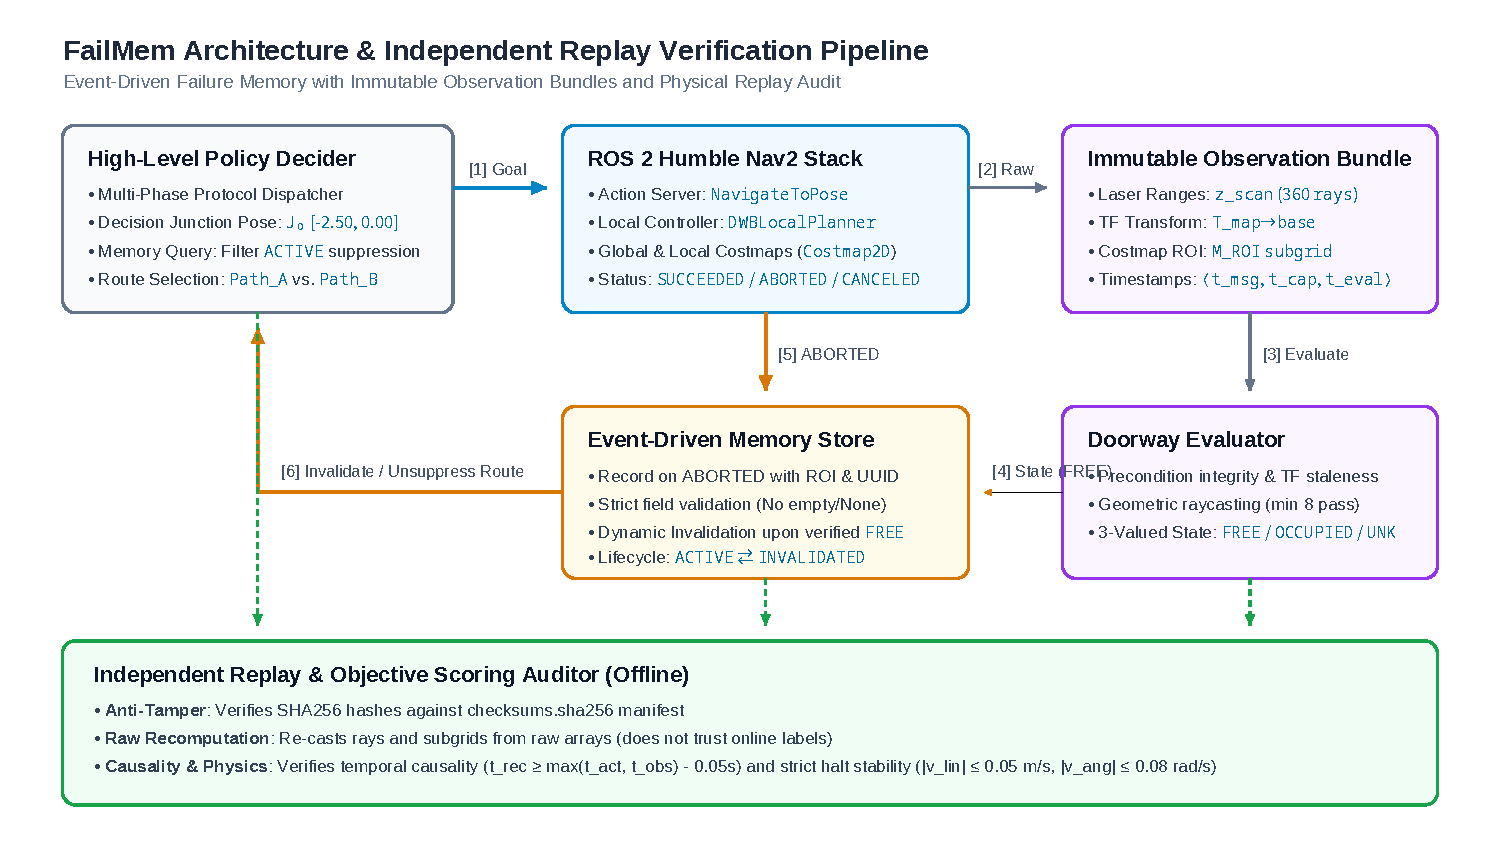
\includegraphics[width=0.85\textwidth]{figures/architecture.pdf}
\caption{FailMem system architecture and verification pipeline, encompassing execution runtime, immutable observation bundles, and memory lifecycle.}
\label{fig:architecture}
\end{figure*}

Figure~\ref{fig:architecture} illustrates the overall system architecture, encompassing the execution runtime, immutable observation bundles, and memory lifecycle.

\subsection{Immutable Observation Bundles}
Prior to evaluating passage clearance, FailMem constructs an immutable observation bundle $B$:
\begin{equation}
B = \langle \text{obs\_id}, \mathbf{z}_{\text{scan}}, \mathbf{T}_{\text{map}\to\text{base}}, \mathbf{M}_{\text{costmap\_ROI}}, t_{\text{msg}}, t_{\text{capture}}, t_{\text{eval}} \rangle
\end{equation}
where $\mathbf{z}_{\text{scan}}$ is the raw range array, $\mathbf{T}_{\text{map}\to\text{base}}$ is the TF transformation, and $\mathbf{M}_{\text{costmap\_ROI}}$ is the extracted 2D subgrid matrix.

\subsection{Clearance Classification Rules}
The passage state is evaluated according to strict geometric criteria implemented in \texttt{src/doorway\_evaluator.py}:
\begin{equation}
\text{State}(B) = \begin{cases} 
\text{OCCUPIED}, & \text{if } N_{\text{hits\_inside}} \ge 5 \text{ or } N_{\text{costmap\_occupied\_cells}} > 0 \\ 
\text{FREE}, & \text{if } N_{\text{hits\_inside}} = 0 \text{ and } N_{\text{pass\_through}} \ge 8 \\
             & \quad \text{and } \text{CostmapCleared}(B) \\ 
\text{UNKNOWN}, & \text{otherwise} 
\end{cases}
\end{equation}
where $\text{CostmapCleared}(B) \iff (N_{\text{unknown\_cells}} = 0 \land N_{\text{occupied\_cells}} = 0)$ within the doorway ROI $[-0.15, 0.15, 0.95, 1.45]$. (See Supplementary Material S1 for detailed transform alignment and ray projection preconditions).

\subsection{Memory Lifecycle \& Invalidation Mechanics}
\begin{itemize}
    \item \textbf{Failure Registration}: When navigation fails within an occupied passage, an active failure record is created:
    \begin{equation}
    M = \langle \text{mem\_id}, t_{\text{fail}}, \text{goal\_uuid}, \text{action\_id}, \text{region\_id}, \mathbf{M}_{\text{costmap\_ROI}} \rangle
    \end{equation}
    Active failure records suppress the associated route at Decision Junction $J_0$.
    \item \textbf{Dynamic Invalidation}: When subsequent sensor perception yields $\text{State}(B) = \text{FREE}$ with evidence timestamp $t_{\text{free}} > t_{\text{fail}}$, the memory entry is marked $\text{INVALIDATED}$, unsuppressing the route.
    \item \textbf{Cross-Phase Scope Clarification}: In the current experimental implementation, history collection, memory creation, decision dispatch, and memory reset occur within a single continuous runner session across sequential phases. This evaluates phase-to-phase memory transfer within an experimental run, and has not yet been benchmarked as a persistent multi-task database across separate OS daemon lifetimes.
    \item \textbf{Evaluation Pipeline}: An independent replay auditor verifies all serialized logs against SHA256 checksum manifests (detecting file changes relative to the manifest) and physical halt stability criteria ($|v_{\text{lin}}| \le 0.05\,\text{m/s}, |v_{\text{ang}}| \le 0.08\,\text{rad/s}$) without reliance on self-reported runtime assertions (detailed in Supplementary Material Section S2).
\end{itemize}


\section{Experimental Setup \& Benchmarking Protocol}
\subsection{Gazebo Simulation Environment \& Geometry}
Simulations are conducted in ROS 2 Humble with Gazebo 11 simulating a TurtleBot3 Waffle robot in an asymmetric dual-path environment (\texttt{configs/p2c\_dualpath\_world.model}).
\begin{itemize}
    \item \textbf{Path A (North Short Path)}: Waypoint polyline length is $6.124\,\text{m}$ from Decision Junction $J_0 [-2.50, 0.00]$ to Goal $[2.50, 0.00]$ through a $0.80\,\text{m}$ doorway chokepoint at $y=1.20$.
    \item \textbf{Path B (South Bypass Detour)}: Waypoint polyline length is $9.105\,\text{m}$ from $J_0$ to Goal via open corridor at $y=-2.40$.
\end{itemize}

\subsection{Distance Metric Definitions}
To evaluate performance across different phases, we define:
\begin{enumerate}
    \item \textbf{Decision Distance ($d_{\text{dec}}$)}: Physical odometry distance traversed during Phase 2 after goal dispatch from Decision Junction $J_0$ (Path B direct: $\approx 7.54\,\text{m}$; Path A direct: $\approx 5.89\,\text{m}$).
    \item \textbf{Total Distance ($d_{\text{tot}}$)}: Cumulative odometry distance spanning both Phase 1 (historical observation/attempt) and Phase 2 (dispatch to goal).
\end{enumerate}

\subsection{Evaluated Scenarios \& Baseline Methods}
\begin{itemize}
    \item \textbf{Scenario D0 (Unobstructed)}: Doorway is clear; robot navigates Path A without prior history.
    \item \textbf{Scenario D1 (Blocked)}: Doorway chokepoint is obstructed by a physical obstacle box. Phase 1 executes the following sequence:
    (i)~\emph{Vantage Navigation}: The robot navigates from Decision Junction $J_0 [-2.50, 0.00]$ to approach vantage waypoint $[-1.00, 1.20, 0.0]$ and captures initial sensor observation bundle;
    (ii)~\emph{Chokepoint Traversal Attempt}: The robot dispatches a genuine Nav2 action attempting chokepoint traversal to $[0.50, 1.20, 0.0]$ with a $15.0\,\text{s}$ timeout;
    (iii)~\emph{Action Termination}: Nav2 execution aborts due to physical obstacle obstruction;
    (iv)~\emph{Failure Memory Creation}: Upon action termination, the robot captures a fresh post-traversal observation bundle confirming \texttt{OCCUPIED}, classifies the failure cause, and commits an active failure memory record (or updates spatial cache $O$);
    (v)~\emph{Structured Return}: The robot executes a return navigation action back to Decision Junction $J_0$.
    Phase 2 then evaluates routing dispatched from $J_0$. Under Reactive $R$, having no cross-phase memory, the robot dispatches the nominal shortest path (Path A), physically travels to entrance waypoint $[-1.50, 1.20]$, detects the blockage on live sensors, and retreats to $J_0$ before taking Path B. This decision-phase unguided probe in $R$ is strictly distinct from the historical Phase 1 traversal attempt executed in $F$ and $O$.
    \item \textbf{Scenario D2 (Cleared)}: Following D1, the obstacle is removed. Phase 1 observes \texttt{FREE} doorway clearance from vantage waypoint $[-1.00, 1.20]$ and retreats to $J_0$. Phase 2 evaluates routing from $J_0$.
\end{itemize}

\textbf{Evaluated Methods}:
\begin{enumerate}
    \item \textbf{Reactive Baseline ($R$)}: No cross-phase memory. In D1, enters Path A approach leg, detects blockage at $[-1.50, 1.20]$, and retreats to $J_0$ before taking Path B.
    \item \textbf{Spatial Observation Cache ($O$)}: Caches 2D geometric occupancy observed from vantage point during Phase 1. Evaluated at $J_0$ during Phase 2.
    \item \textbf{FailMem ($F$)}: Event-driven failure memory with dynamic perception-driven invalidation.
    \item \textbf{Persistent Suppression ($M1$)}: Static failure memory permanently suppressing Path A without dynamic invalidation.
\end{enumerate}

All runs use $n=3$ per condition under sequential fixed seeds with an episode simulation time budget of $180.0\,\text{s}$, yielding 30 Gazebo simulation runs in total.


\section{Empirical Results \& Boundary Analysis}
\subsection{Condition-Level Performance}
Table~\ref{tab:condition_summary} presents condition-level performance across 30 Gazebo simulation runs ($n=3$ per condition, reporting mean $\pm$ sample standard deviation with Bessel correction $ddof=1$). All 10 conditions achieved a $100\%$ replay audit pass rate ($3/3$), confirming physical halt stability and data completeness across all runs.

\begin{table*}[t]
\centering
\caption{Condition-Level Navigation Performance Across 30 Gazebo Simulation Runs ($n=3$ per condition, mean $\pm$ sample std dev, $ddof=1$).}
\label{tab:condition_summary}
\resizebox{\textwidth}{!}{%
\begin{tabular}{llclcccccc}
\hline
Scenario & Method & $n$ & Actual Route & Dead-Ends & Decision Dist (m) & Decision Time (s) & Total Dist (m) & Total Time (s) & Replay Audit Pass \\
\hline
D0 & R & 3 & Path\_A & 0.0 $\pm$ 0.0 & 6.16 $\pm$ 0.04 & 51.5 $\pm$ 1.7 & 6.16 $\pm$ 0.04 & 51.5 $\pm$ 1.7 & 3/3 (100\%) \\
D0 & O & 3 & Path\_A & 0.0 $\pm$ 0.0 & 6.20 $\pm$ 0.01 & 50.0 $\pm$ 0.8 & 6.20 $\pm$ 0.01 & 50.0 $\pm$ 0.8 & 3/3 (100\%) \\
D0 & F & 3 & Path\_A & 0.0 $\pm$ 0.0 & 6.20 $\pm$ 0.03 & 49.9 $\pm$ 0.5 & 6.20 $\pm$ 0.03 & 49.9 $\pm$ 0.5 & 3/3 (100\%) \\
D1 & R & 3 & Path\_A\_then\_Path\_B & 1.0 $\pm$ 0.0 & 10.82 $\pm$ 0.07 & 82.1 $\pm$ 4.4 & 17.22 $\pm$ 0.24 & 141.0 $\pm$ 5.9 & 3/3 (100\%) \\
D1 & O & 3 & Path\_B & 0.0 $\pm$ 0.0 & 7.55 $\pm$ 0.05 & 50.0 $\pm$ 2.0 & 13.95 $\pm$ 0.07 & 108.7 $\pm$ 2.7 & 3/3 (100\%) \\
D1 & F & 3 & Path\_B & 0.0 $\pm$ 0.0 & 7.54 $\pm$ 0.00 & 48.2 $\pm$ 1.0 & 14.03 $\pm$ 0.25 & 109.5 $\pm$ 1.6 & 3/3 (100\%) \\
D2 & R & 3 & Path\_A & 0.0 $\pm$ 0.0 & 5.92 $\pm$ 0.04 & 49.6 $\pm$ 1.6 & 16.34 $\pm$ 0.03 & 148.2 $\pm$ 3.2 & 3/3 (100\%) \\
D2 & O & 3 & Path\_A & 0.0 $\pm$ 0.0 & 5.94 $\pm$ 0.07 & 52.0 $\pm$ 1.7 & 16.40 $\pm$ 0.24 & 149.8 $\pm$ 0.6 & 3/3 (100\%) \\
D2 & F & 3 & Path\_A & 0.0 $\pm$ 0.0 & 5.89 $\pm$ 0.02 & 51.1 $\pm$ 1.0 & 16.25 $\pm$ 0.10 & 151.1 $\pm$ 7.8 & 3/3 (100\%) \\
D2 & M1 & 3 & Path\_B & 0.0 $\pm$ 0.0 & 7.89 $\pm$ 0.02 & 51.3 $\pm$ 2.0 & 18.25 $\pm$ 0.09 & 148.8 $\pm$ 2.4 & 3/3 (100\%) \\
\hline
\end{tabular}%
}
\end{table*}


\subsection{Pairwise Contrasts \& Trajectory Analysis}
Table~\ref{tab:pairwise_contrasts} reports pairwise contrast comparisons across evaluated methods, and Figure~\ref{fig:trajectories} illustrates representative trajectories from the Gazebo simulation runs.

\begin{table}[t]
\centering
\footnotesize
\caption{Key Pairwise Contrasts Between Methods Across Scenarios D1 and D2.}
\label{tab:pairwise_contrasts}
\setlength{\tabcolsep}{2.5pt}
\begin{tabular}{lllcccc}
\toprule
Scenario & Contrast & Metric & $A$ & $B$ & \shortstack{Diff\\($A-B$)} & \shortstack{Rel\\(\%)} \\
\midrule
D1 & $F$ vs. $R$  & Dist (m) & 14.03  & 17.22  & -3.19  & -18.5\% \\
D1 & $F$ vs. $R$  & Time (s) & 109.50 & 141.00 & -31.50 & -22.3\% \\
D1 & $O$ vs. $R$  & Dist (m) & 13.95  & 17.22  & -3.27  & -19.0\% \\
D1 & $O$ vs. $R$  & Time (s) & 108.70 & 141.00 & -32.30 & -22.9\% \\
D1 & $F$ vs. $O$  & Dist (m) & 14.03  & 13.95  & +0.08  & +0.6\%  \\
D1 & $F$ vs. $O$  & Time (s) & 109.50 & 108.70 & +0.80  & +0.7\%  \\
D2 & $F$ vs. $M1$ & Dist (m) & 16.25  & 18.25  & -2.00  & -11.0\% \\
D2 & $F$ vs. $M1$ & Time (s) & 151.10 & 148.83 & +2.27  & +1.5\%  \\
D2 & $F$ vs. $O$  & Dist (m) & 16.25  & 16.40  & -0.15  & -0.9\%  \\
D2 & $F$ vs. $O$  & Time (s) & 151.10 & 149.77 & +1.33  & +0.9\%  \\
\bottomrule
\end{tabular}
\end{table}


\begin{figure}[t]
\centering
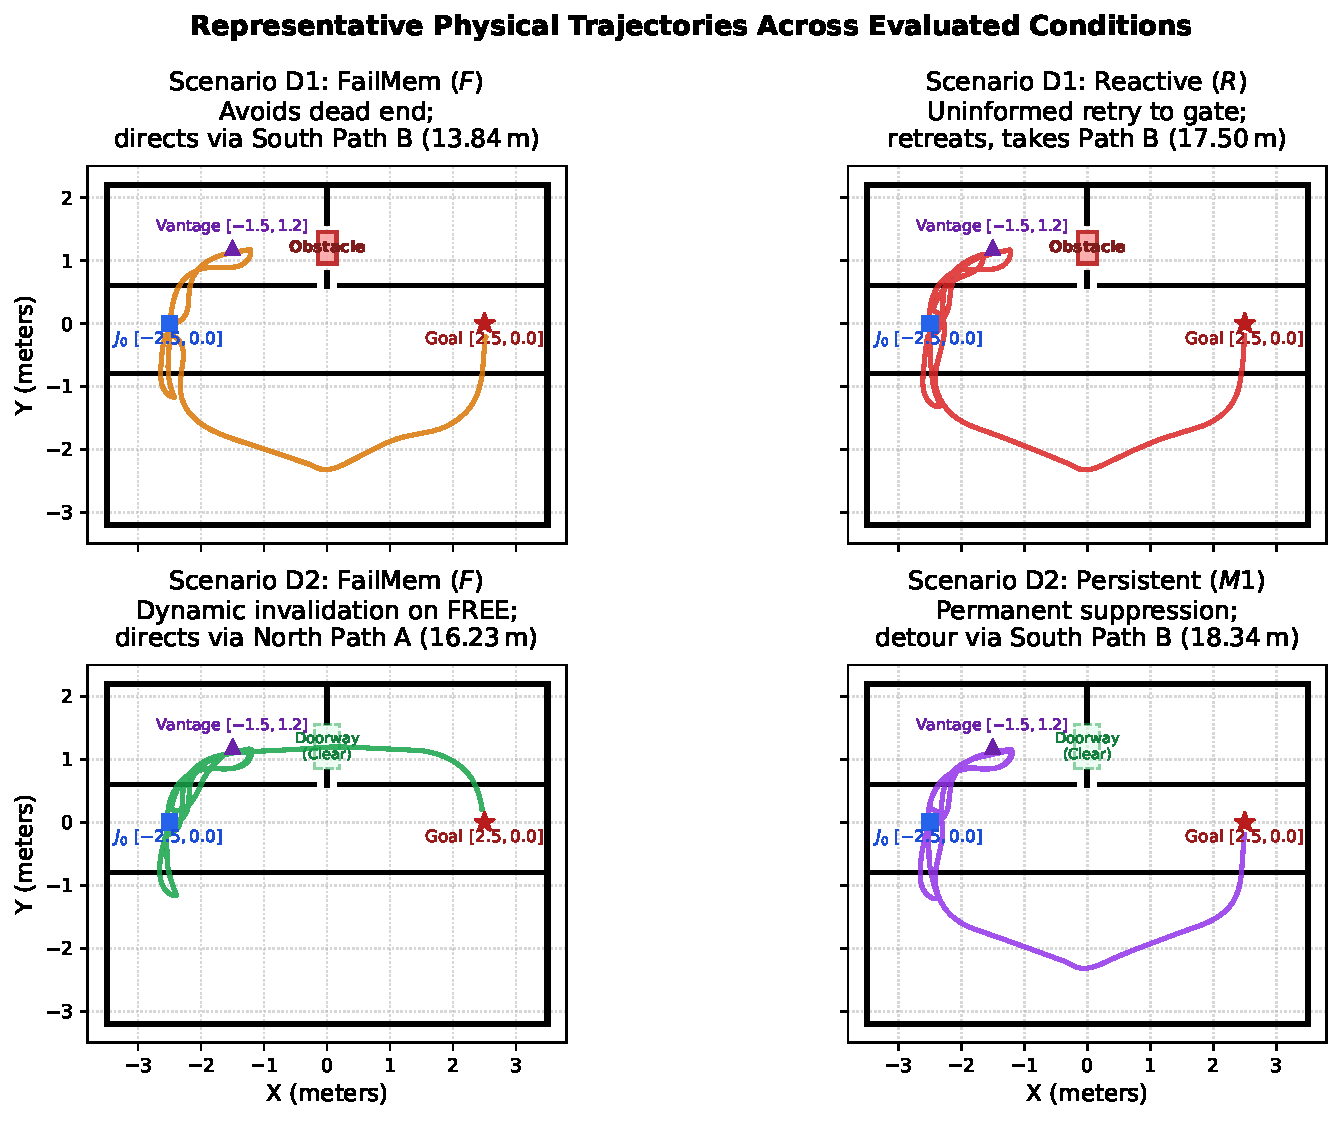
\includegraphics[width=\columnwidth]{figures/trajectories_map.pdf}
\caption{Representative Gazebo simulation trajectories across evaluated conditions.}
\label{fig:trajectories}
\end{figure}

\begin{enumerate}
    \item \textbf{Elimination of Redundant Dead-End Exploration ($F$ vs. $R$)}: In Scenario D1, FailMem ($F$) eliminates redundant entry into the blocked corridor ($0.0$ vs. $1.0$ dead ends), reducing total distance by $-18.5\%$ ($14.03\,\text{m}$ vs. $17.22\,\text{m}$) and simulation duration by $-22.3\%$ ($109.5\,\text{s}$ vs. $141.0\,\text{s}$) relative to Reactive $R$ (Table~\ref{tab:pairwise_contrasts}, Figure~\ref{fig:trajectories}). Reactive $R$'s dead-end traversal represents an unguided retry to the entrance waypoint, not collision.
    \item \textbf{Prevention of Detour Overhead ($F$ vs. $M1$)}: In Scenario D2, dynamic invalidation upon observing \texttt{FREE} unsuppresses Path A, reducing total distance by $\approx 11.0\%$ ($2.00\,\text{m}$, $16.25\,\text{m}$ vs. $18.25\,\text{m}$) relative to persistent suppression ($M1$). However, in the current 3-run exploratory evaluation, average total simulation duration showed no observed improvement and increased slightly by $\approx 1.5\%$ ($151.1\,\text{s}$ vs. $148.8\,\text{s}$, a sample mean difference of $+2.27\,\text{s}$). An independent three-phase trajectory time ledger analysis reveals the empirical source of this discrepancy: the $+2.27\,\text{s}$ full-episode duration sample mean difference was accrued predominantly during the \textbf{History Exploration Phase} ($t < T_{\text{history}}$), where FailMem took $100.00 \pm 7.72\,\text{s}$ vs. $M1$'s $97.53 \pm 2.12\,\text{s}$ (a $+2.47\,\text{s}$ exploration sample mean difference accrued prior to route dispatching). During the \textbf{Decision Phase} ($t \ge T_{\text{history}}$), execution durations between FailMem and $M1$ were virtually identical ($51.10 \pm 0.95\,\text{s}$ vs. $51.30 \pm 2.00\,\text{s}$, a difference of only $-0.20\,\text{s}$), indicating no observable end-to-end time advantage for Path A in this benchmark. An exploratory kinematic decomposition shows that along Path A, active moving time was shorter ($28.70 \pm 1.18\,\text{s}$ vs. $34.30 \pm 1.76\,\text{s}$ at default thresholds, a sample mean difference of $-5.60\,\text{s}$), reflecting shorter path length ($5.89\,\text{m}$ vs. $7.89\,\text{m}$), while stopped time was longer ($15.83 \pm 2.42\,\text{s}$ vs. $12.13 \pm 1.41\,\text{s}$, a sample mean difference of $+3.70\,\text{s}$), alongside independent doorway clearance settling window measurements ($6.97 \pm 0.06\,\text{s}$ vs. $4.60 \pm 0.00\,\text{s}$). Because component durations vary with discretization thresholds (active moving difference spans $-5.10\,\text{s}$ to $-6.80\,\text{s}$ and stationary difference spans $+3.10\,\text{s}$ to $+5.20\,\text{s}$ across linear velocity thresholds $0.03\text{--}0.08\,\text{m/s}$ in our sensitivity analysis, Supplementary Material Section S5), we report these as coarse-grained observational latencies rather than asserting an invariant physical mechanism.
    \item \textbf{Comparison with Spatial Caching in Static 2D Geometry ($F$ vs. $O$)}: In both D1 and D2, FailMem ($F$) and Spatial Cache ($O$) selected identical topological routes. Total distance differences ($+0.6\%$ in D1, $-0.9\%$ in D2) and total duration differences ($+0.7\%$ in D1, $+0.9\%$ in D2) remained under $1\%$. In the evaluated static 2D hallway layout, specific implementation, and run sample ($n=3$), no additional routing benefit of $F$ over $O$ was observed; this does not imply general lack of benefit across arbitrary domains or statistical equivalence. Notably, dynamic recovery upon obstacle removal is not exclusive to FailMem; spatial costmap caching ($O$) likewise updates its internal occupancy state and unblocks routes upon acquiring new sensory observations.
\end{enumerate}

\subsection{Feasibility Check for Action-Conditioned Navigation ($H_1$)}
To investigate whether action configurations (aligned $a_{\text{aligned}}$ vs. doorpost boundary-biased oblique $a_{\text{oblique}}$) create executability differences in an unobstructed doorway, a fixed 4-run feasibility check was conducted.

\begin{table*}[t]
\centering
\footnotesize
\caption{Exploratory Feasibility Results for Action-Conditioned Navigation Hypothesis $H_1$ ($n=4$).}
\label{tab:h1_feasibility}
\setlength{\tabcolsep}{3.0pt}
\begin{tabular*}{\textwidth}{@{\extracolsep{\fill}}llcccccccc@{}}
\toprule
Run Name & Profile & Target Goal & Perception & Nav2 Status & \shortstack{Nav2\\Time (s)} & \shortstack{Settling\\(s)} & \shortstack{Stability\\(s)} & \shortstack{Total\\Sim (s)} & Strict Arrival \\
\midrule
H1\_aligned\_run1 & act\_aligned & [1.50, 1.20] & FREE (23) & SUCCEEDED (4) & 13.4 & 3.0 & 2.4 & 18.8 & \shortstack{\textbf{False}\\\scriptsize($\omega_{\text{ang}}: 0.107 > 0.08$)} \\
H1\_aligned\_run2 & act\_aligned & [1.50, 1.20] & FREE (22) & SUCCEEDED (4) & 13.4 & 3.0 & 2.4 & 18.8 & \textbf{True} \\
H1\_oblique\_run1 & act\_oblique & [0.50, 0.88] & FREE (23) & SUCCEEDED (4) & 11.1 & 3.0 & 2.3 & 16.4 & \textbf{True} \\
H1\_oblique\_run2 & act\_oblique & [0.50, 0.88] & FREE (22) & SUCCEEDED (4) & 11.0 & 3.0 & 2.3 & 16.3 & \textbf{True} \\
\bottomrule
\end{tabular*}
\end{table*}


Table~\ref{tab:h1_feasibility} summarizes the feasibility trial outcomes. Nav2 returned \texttt{SUCCEEDED} (status code 4) in all 4/4 runs, and strict physical arrival was verified in 3/4 runs (\texttt{H1\_aligned\_run1} exceeded the angular velocity halt threshold during the stability window: $0.1068 > 0.08\,\text{rad/s}$). Nav2's \texttt{DWBLocalPlanner} navigated the passage without planner abortion across all runs.

\textbf{Decision \& Conclusion}: \emph{Nav2 returned success in 4/4 runs, with strict physical arrival verified in 3/4 runs; the candidate scenario did not establish the expected executability divergence. Exploration for this hypothesis was therefore stopped per protocol, which does not constitute a refutation of the general action-conditioned failure memory hypothesis.}


\section{Threats to Validity \& Limitations}
\begin{enumerate}
    \item \textbf{Exploratory Sample Size}: The 30-run comparative pilot ($n=3$ per condition) serves as an exploratory demonstration of mechanism functioning and auditability; it does not constitute large-sample asymptotic hypothesis testing.
    \item \textbf{Simulation Fidelity}: Evaluated in Gazebo 11 simulation with nominal sensor models. Physical robot hardware deployments with real-world sensor dropout, dynamic obstacles, and adversarial conditions are subject to future research.
    \item \textbf{Conceptual Extensions ($F2, O+$)}: Action-profiled failure memory ($F2$) and backoff spatial caching ($O+$) are formalized as conceptual models in project documentation but have not yet been evaluated in simulation.
    \item \textbf{Within-Session Phase-Level Scope}: Memory evaluation is restricted to sequential phases within a single continuous experimental execution session. Cross-task persistence across operating system restarts, long-term storage indexing, and multi-day operation remain unverified.
\end{enumerate}


\section{Conclusion}
This paper presented FailMem, an event-driven failure memory architecture for autonomous mobile robots. By binding execution failures to immutable observation bundles and providing an independent replay audit pipeline, FailMem establishes rigorous standards for reproducible robotics evaluation. Our empirical findings demonstrate that historical information eliminates redundant dead-end exploration relative to reactive retry, and dynamic state updates (available in both FailMem and spatial caching) prevent permanent detour traps upon environmental recovery. In the evaluated layout and run sample, no additional routing benefit of explicit failure memory over spatial caching was observed. These findings provide an auditable, reproducible benchmark and empirical stopping rationale to guide future research on action-conditioned and multi-agent memory systems.


\section*{Acknowledgment}
\noindent [Funding Grant Placeholder: This work was supported by Grant Placeholder \texttt{\#XXXX-XXXX} from Funding Agency Placeholder. Compute resources were provided by Institution Placeholder.]

\bibliographystyle{ieeetr}
\bibliography{references}

\end{document}
